\newpage

\section*{Task 6}
In this section, a D Flip-Flop and a SR Latch
are implemented, based on logic gates.
\subsection*{SR Latch}
For the SR Latch, it is 
implemented using NOR gates of 74HC02 integrated
circuit. The resulting schematic is shown below.

\begin{figure}[H]
    \begin{centering}
    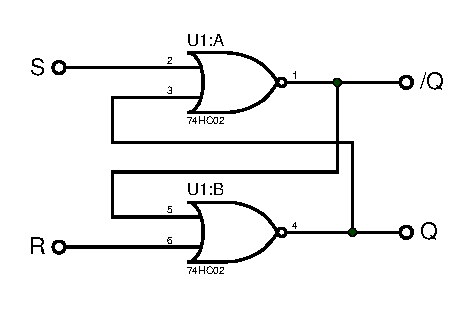
\includegraphics[width=0.4\textwidth]{data/latchSR}
    \par\end{centering}
    \caption{SR Latch circuit - Made in Proteus 7.8}
\end{figure}

PARAMETROS IMPORTANTES: PROPAGACION DE SET O 
RESET A LAS SALIDAS. MEDIR. COMPARAR CON UNO
COMERCIAL CUALQUIERA

\begin{table}[H]
    \begin{center}
        \begin{tabular}{|c|c|c|c|c|}
            \hline 
            \multicolumn{2}{|c|}{PARAMETER} & FROM & TO & VALUE\tabularnewline
            \hline 
            \hline 
            \multirow{2}{*}{$t_{pd}$} & Circuit & S & Q & \tabularnewline
            \cline{2-5} 
             & 74HC279 & S & Q & 30ns o 26ns\tabularnewline
            \hline 
            \multirow{2}{*}{$t_{pd}$} & Circuit & R & Q & \tabularnewline
            \cline{2-5} 
             & 74HC279 & R & Q & 31ns o 36ns\tabularnewline
            \hline 
            \end{tabular}
    \caption{Measured values}
    \end{center}
\end{table}

\subsection*{D Flip-Flop}
For the D flip-flop, it is implemented using 
the SR Latch designed before, adding the 
remaining parts as shown below.

\begin{figure}[H]
    \begin{centering}
    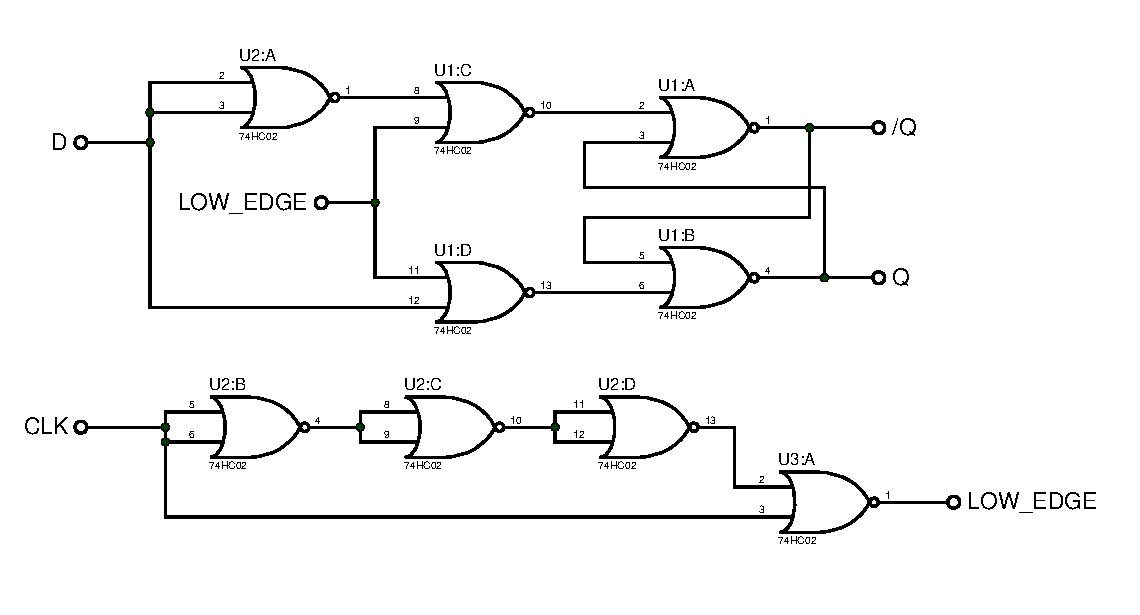
\includegraphics[width=0.9\textwidth]{data/dflipflop}
    \par\end{centering}
    \caption{D Flip-Flop circuit - Made in Proteus 7.8}
\end{figure}

PARAMETROS IMPORTANTES: PROPAGACION DEL D A
LA SALIDA LUEGO DEL CLK, TANTO PARA 0 COMO
PARA 1. MEDIR. COMPARAR CON UNO COMERCIAL
CUALQUIERA.
The designed circuit will be compared with the 
74HC74 D Flip-Flop, using the datasheet of Texas 
Instruments.

\begin{table}[H]
    \begin{center}
        \begin{tabular}{|c|c|c|c|c|}
            \hline 
            \multicolumn{2}{|c|}{PARAMETER} & FROM & TO & VALUE\tabularnewline
            \hline 
            \hline 
            \multirow{2}{*}{$t_{pd}$} & Circuit & CLK & Q or /Q & \tabularnewline
            \cline{2-5} 
             & 74HC74 & CLK & Q or /Q & 44ns o 37ns\tabularnewline
            \hline 
            \multirow{2}{*}{$t_t$} & Circuit &  & Q or /Q & \tabularnewline
            \cline{2-5} 
             & 74HC74 &  & Q or /Q & 19ns o 16ns\tabularnewline
            \hline 
            \end{tabular}
    \caption{Measured values}
    \end{center}
\end{table}

